\section {Formularea problemei}

In orase precum Bucuresti, majoritatea blocurilor au fost contruite inainte de anul 1990 si prin urmare interfoanele lor se bazeaza pe \acrshort{pots}. Traind in era digitala, utilizatorul ideal (e corporatist) isi doreste augmentarea functionalitatilor sistemului existent, pentru a nu trebui sa isi convinga toti vecinii sa investeasca in modernizarea sistemului de acces. Pentru a putea adresa cat mai multi utilizatori, solutia acestei probleme trebuie sa fie agnostica de smartphoneul si interfonul existent a utilizatorului, dar sa ofere integrari cu alte solutii de tip "Smart Home".

In functie de perioada instalarii, sistemele sa impart in doua categorii: analogice si digitale. Posturile de interfon analogice sunt legate la o unitate de comanda care decodeaza semnale \acrfull{dtmf}, genereaza un semnal sinusoidal cu frecventa de 20Hz si amplitudinea de 60-90V pentru sonerie, apoi realizeaza conexiunile necesare dintre postul de afara si cel al apartamentului cautat. Sistemele digitale folosesc o magistrala comuna de comunicatii, fiind adresate conform unei scheme prestabilite - fiecare terminal este programat cu o adresa, insa pentru acest procedeu este nevoie de o cheie asociata unitatii de comanda.

Din motive istorice, standardul unitatea centrala \acrshort{pots} genereaza semnalul sinusoidal si poarta suficient curent pentru a putea alimenta clopotul aparut cu prima generatie de telefoane. Prin urmare, sistemele digitale sunt considerate mai eficiente si mai sigure, dar si mai greu de integrat, datorita implicarii unei persoane autorizate care sa programeze intregul sistem.

Aceasta lucrare va analiza solutii digitale, insa sistemul final va fi implementat impreuna cu un terminal analog. Asadar, trebuie sa intelegem in primul rand mecanismul de adresare si cum este el interpretat de centrala. Dupa cum insinueaza numele, \acrshort{dtmf} presupune generarea a doua tonuri de frecevente diferite in acelasi timp, conform liniei si coloanei tastei apasate. Acest semnal va fi intrepretat de decodorul de semnal al centralei cu ajutorul unor filtre de tip notch spre a se realiza conexiunile necesare. 

\begin{table}[ht!]
\begin{tabular}{c||c|c|c}
 & 1209Hz & 1336Hz & 1477Hz \\
\hline
\hline
697Hz & 1 & 2 & 3 \\
\hline
770Hz & 4 & 5 & 6 \\
\hline
852Hz & 7 & 8 & 9 \\
\hline
941Hz & * & 0 & \# \\
\end{tabular}
\centering
\caption{Tabel frecvente \acrshort{dtmf}}
\label{tab:dtmf}
\end{table}

Sistemul descris pana acum poate adresa $12-1=11$ posturi diferite (centrala este considerata si ea post si are un slot rezervat). Pentru a adresa mai multe posturi, unitatea de comanda trebuie sa includa si un circuit logic secvential pentru a retine starea ultimelor taste apasate. Astfel, ajungem la un numar satisfacator de adrese pentru aplicatia interfonului. 

Un exemplu de analiza spectrala a unui astfel de semnal:

\begin{figure}[h!]
  \centering
  \fbox {
    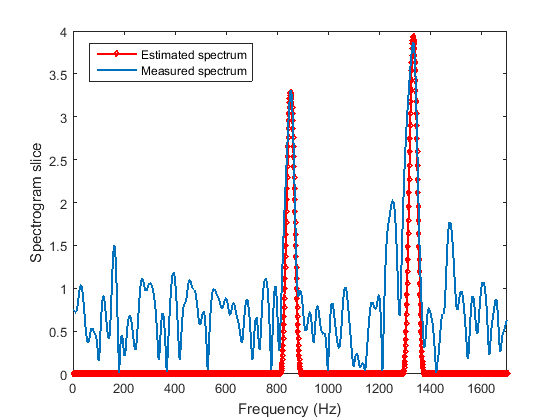
\includegraphics[width=\singlefigure]{02/04_spectru_dtmf.png}  
  }
  \caption{Spectrograma tasta "8" \cite{AunsriNattapol2016}}
\end{figure}

Se pot distinge grafic doua frecvente predominante: 852Hz si 1336Hz - cobinatia corespunaztoare tastei "8".

\section {Studiu asupra realizărilor similare din domeniu}


\subsection {Videx UK}

Interfoanele \acrshort{gsm} de la Videx sunt conectate la reteaua mobila de telefonie si permit operarea unei porti prin intermediul unui releu. Ele necesita doar o sursa de curent externa, o antena si o cartela \acrfull{sim} pentru a opera.

\begin{figure}[h!]
  \centering
  \fbox {
    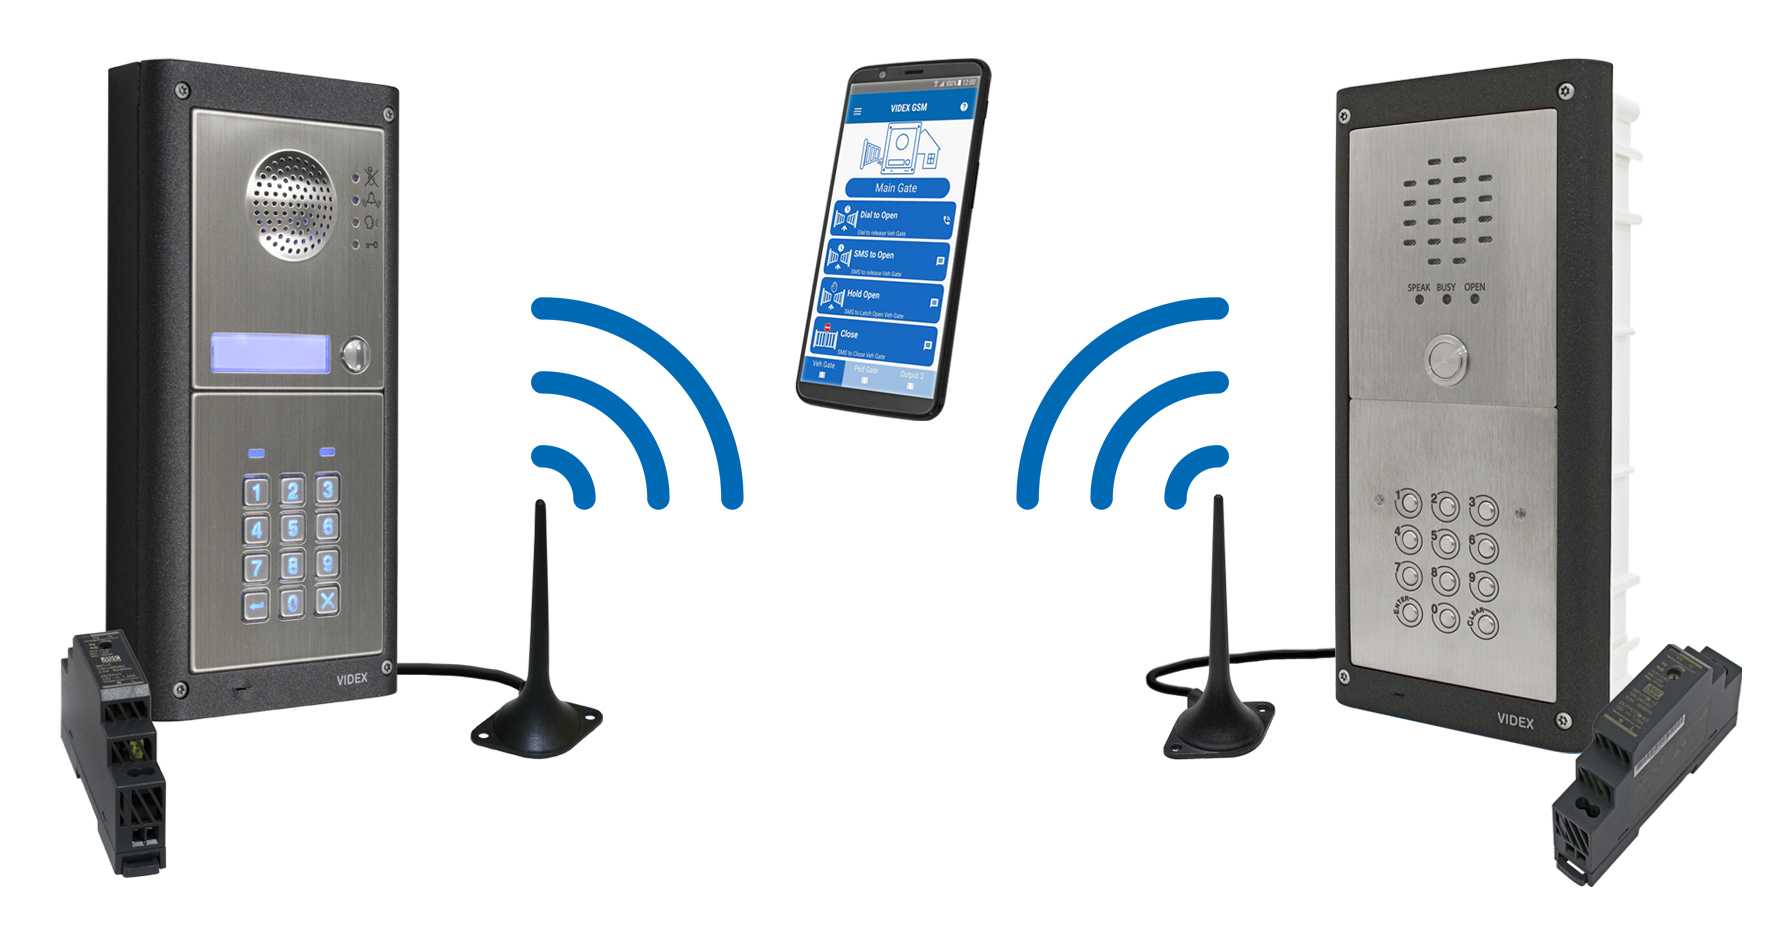
\includegraphics[width=\singlephoto]{02/01_gsm_system.jpg}  
  }
  \caption{Sistem interfon Videx GSM \cite{VidexUk}}
\end{figure}

Printre functionalitatile principale se numara:
\begin{itemize}
  \item Poate include un cititor de carduri \acrshort{rfid} si cheie
  \item Versiune rezistenta la vandalism
  \item Pana la 4 numere de telefon per apartament, pentru redundanta. In cazul in care primul numar nu se poate apela sau nu raspunde, se va incerca urmatorul numar programat
  \item Ofera aplicatie Android si iOS pentru programat unitatea
\end{itemize}

Dezavantaje:

\begin{itemize}
  \item Nu ofera integrare cu servicii din reteaua \acrshort{iot}
\end{itemize}

\subsection {Google Nest x Yale Lock}

\begin{figure}[h!]
  \centering
  \fbox {
    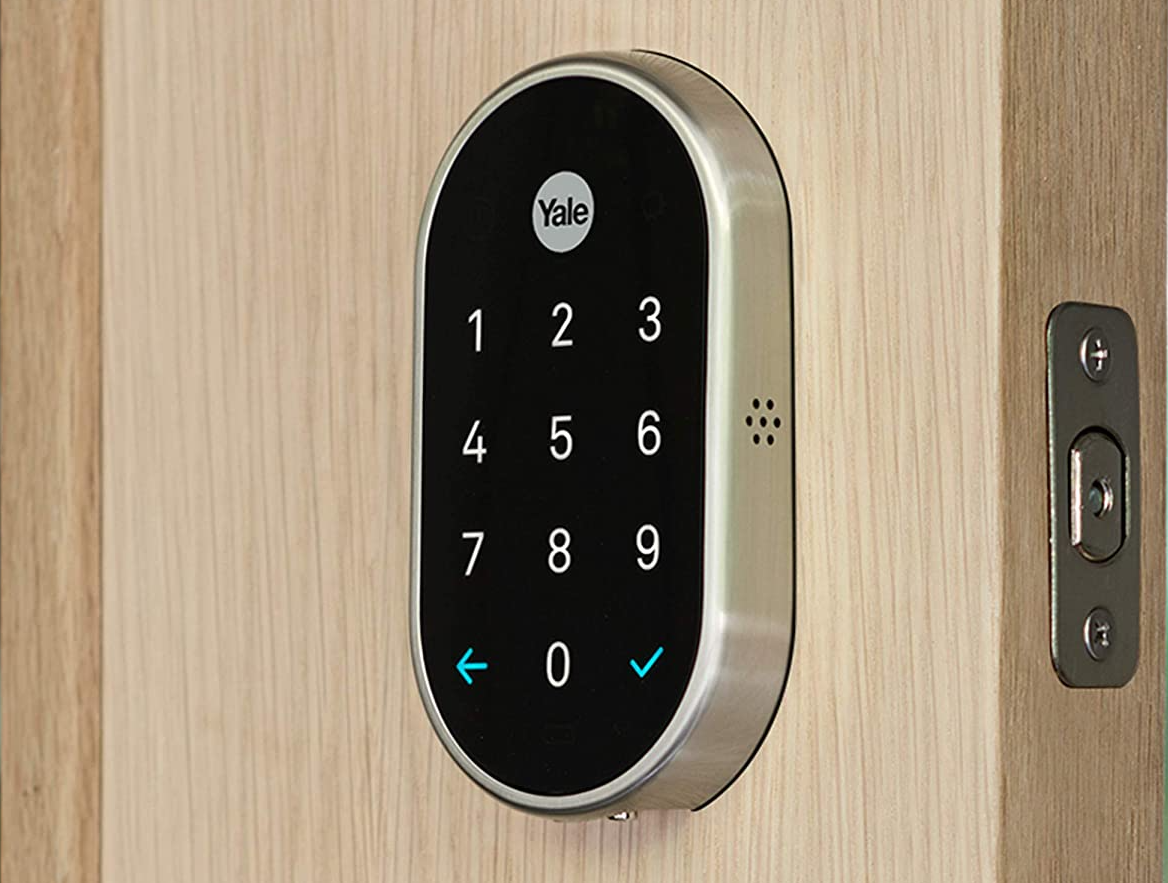
\includegraphics[width=\singlephoto]{02/02_iot_system.png}  
  }
  \caption{Next x Yale Lock \cite{YaleLock}}
\end{figure}

Avantaje:
\begin{itemize}
  \item Permite accesul prin intermediul unui PIN ales de utilizator
  \item Ofera alerte cand cineva inchide sau deschide usa
  \item Ofera integrare cu Google Home si Nest Home
\end{itemize}

Dezavantaje:
\begin{itemize}
  \item Are nevoie de 4 baterii tip AA pentru a functiona
  \item Nu are acces cu cheie sau cartela
  \item Nu are versiune rezistenta
\end{itemize}


\subsection {Level Lock - Touch Edition}

Level Lock este o incuietoare inteligenta de tip zavor. Are un design minimalist si ascunde partea electronica in interiorul usii pentru mai multa securitate.

\begin{figure}[h!]
  \centering
  \fbox {
    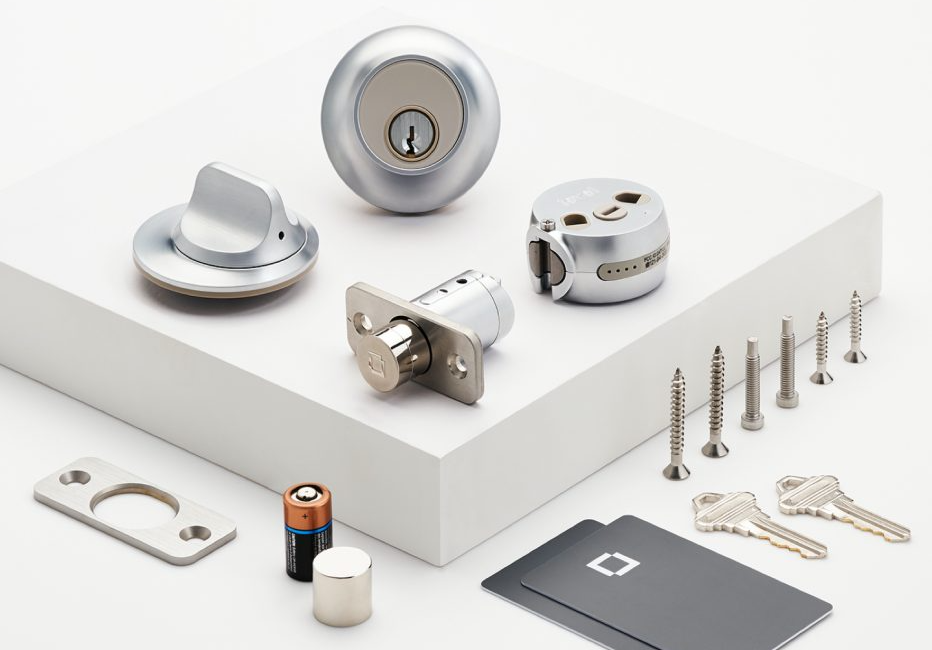
\includegraphics[width=\singlephoto]{02/03_iot_system.jpg}  
  }
  \caption{Level Lock \cite{LevelLock}}
\end{figure}

Avantaje:
\begin{itemize}
  \item Multiple modalitati de acces, printre care: amprenta, PIN
  \item Ofera alerte cand cineva inchide sau deschide usa
  \item Ofera integrare cu Google Home si Nest Home
\end{itemize}

\subsection {Comparatii}

Produsele de mai sus adreseaza probleme usor diferite, dar incearca sa ofere functionalitati similare. Sistemul oferit de Videx Security prezinta un design rezistent, dar familiar tuturor utilizatorilor si este destinat cladirilor cu mai multi locatari. In contrast, cele doua incuietori inteligente ofera o integrare avansata in reteaua \acrshort{iot} si multiple cai de acces, dar sunt destinate unei singure locuinte.

Incuietoarea de la Yale prezinta cea mai inovativa abordare a acestul design prin decizia deliberata de a nu oferi posibilitatea de acces cu cheie. Astfel, simplifica partea mecanica eliminand singura cale de acces din exterior catre mecanismul incuietorii.

Produsul celor de la Videx Security se bazeaza pe o tehnologie utilizata la scara larga si prin urmare beneficiaza de robustetea unui sistem matur. Spre deosebire de celelalte doua produse analizate, solutia celor de la Videx Security este agnostica de sistemul de operare al telefonului mobil, avand nevoie doar de o conexiune \acrshort{gsm}.

Din lipsa unor standarde in domeniu, dispozitivele noi sufera de alte tipuri de probleme si vulnerabilitati, dupa un studiu realizat de cercetatorii de la Bitdefender. Majoritatea sunt in faza initiala de setare, oferind protocoale de securitate invechite sau omitandu-le complet. Este mentionat si un dispozitiv care expune un port Telnet, un protocol invechit si usor de exploatat, fara posibilitatea de a fi dezactivat \cite{Bitdefender2016IoT}.

\section {Stabilirea cerințelor funcționale si nefuncționale ale sistemului}
// todo: impartit in functionale/nefunctionale

\subsection{Controlul accesului intr-un apartament}

Scopul principal al acestui sistem este de a oferi sau nu acces intr-o incinta, prin urmare consider aceasta cea mai importanta cerinta functionala.

\subsection{Expunerea unui serviciu REST pentru interfatarea cu alte sisteme}

Expunerea si abstractizarea terminalului \acrshort{pots} este realizata printr-un set de servicii \acrfull{rest} care controleaza starea sa. Acest lucru ne permite interfatarea cu aplicatia mobila, interfata de administrare web si alte servicii precum Google Home/Google Assistant/Apple HomeKit.

\subsection{Implementarea unei functii pentru raspuns automat}

Aceasta functie va permite utilizatorului sa stabileasca o perioada de timp pentru care sistemul va oferi accesul neconditionat.

\subsection{Dezvoltarea unui client mobil Android}

Principalul client care va interactiona cu serviciile \acrshort{rest} va fi aplicatia mobila ce va avea rolul de a notifica userul cand ii suna interfonul si de a controla starea sistemului.

\subsection{Control granular asupra datelor stocate}

Arhitectura aplicatiei necesita interactiunea cu o baza de date, care poate fi tinuta in cloud, pentru convenabilitate sau local.
Folosind tehnologii de containerizare precum Docker, putem stoca baza de date local, informatiile fiind stocate intr-un mediu controlat.

\subsection{Criptarea comunicatiilor cu serviciile web}

Avand in vedere nivelul de acces pe care l-ar oferi un exploit al acestei solutii, comunicatiile intre server si clienti trebuie realizate printr-un canal criptat de tip \acrfull{ssl}. Credentialele userului si ulterior tokenul de acces trebuie trimise doar dupa verificarea autenticitatii serverului si a pachetelor trimise.

\subsection{Oferirea si revocarea accesului la sistem}

Dorim de exemplu sa oferim acces neconditionat unui prieten apropiat pentru a intra in bloc fara a mai suna la interfon. De asemenea ar trebui sa putem realiza si inversul acestei operatii.

\subsection{Expunerea unui flux duplex audio prin tehnologia VoIP}

Pasul final in dezvoltarea acestui sistem ar fi interfatarea cu un \acrfull{adc} si un \acrfull{dac} si expunerea streamurilor de date prin \acrfull{voip}
